\chapter{Accessible Typesetting for Science and Mathematics}
\section{Equations and Mathematical Content}
This template is set up so that equations may be read properly with a screen reader.
Generally, no additional work is required by a \textit{user} of this template.
For example, Eq.~\eqref{eq:basel} is written using standard \LaTeX:
\begin{equation}
  \label{eq:basel}
  \sum\nolimits_{n\in \mathbb{Z}^+} \frac{1}{n^2}
  = \frac{\pi^2}{6}
  \approx 1.6449.
\end{equation}
Despite this, there are several known bugs concerning how equations are tagged and read on a screen reader.
The \texttt{lualatex} compiler is generally quite good about warning you when you encounter one of these bugs; however, you are encouraged to manually inspect your final PDF using the resources mentioned in \autoref{sec:checkers}, as equations which are typeset correctly in your PDF may not display correctly in the associated MathML (and thus on a screen reader).
For example, there is a \href{https://github.com/latex3/tagging-project/issues/1033}{known bug} concerning how split equations are tagged.
If you have a particularly long equation that needs to be split over multiple lines, you are advised to use the \texttt{align} environment instead of \texttt{split}, as in Eq.~\eqref{eq:align-example} for example.
\begin{align}
  \label{eq:align-example}
  \frac{d^5W}{d\Omega_e d\Omega_\nu dE_e}
  = \frac{G_F^2|V_{ud}|^2}{2\pi^5}p_eE_e(A_0-E_e)^2
  % 
  &\,\xi\left[1+a_{\beta\nu}\frac{\symbf{p}_e\cdot\symbf{p}_\nu}{E_eE_\nu}+b\frac{\Gamma m_e}{E_e}\right.\nonumber\\
  &\qquad\left.+\frac{\symbf{I}}{I}\cdot\left(A_\beta\frac{\symbf{p}_e}{E_e}+B_\nu\frac{\symbf{p}_\nu}{E_\nu}+D\frac{\symbf{p}_e\times\symbf{p}_\nu}{E_e E_\nu}\right)\right].
\end{align}
Pursuant to these accessibility goals, this template uses the \texttt{unicode-math} package, which enables Unicode mathematical input and OpenType math fonts.
The downside of this, however, is that some legacy math font packages may be unnecessary or incompatible, or may not work as expected in this template.
If you encounter any difficulty incorporating any of your existing work into this template, please refer to the troubleshooting tips in \ref{appx:troubleshoot}.

As a final note, you are advised to avoid numbering equations of minor importance and to use \verb|\eqref| to reference equations in-text, so that these references may be formatted as in the previous example.

\section{Algorithms, Code, and Pseudocode}
Common packages for generating pseudocode such as \texttt{algorithm2e} and \texttt{algorithm} are currently incompatible with PDF tagging; however, simpler packages such as \texttt{algpseudocode} work at this time:

\noindent
\rule{\textwidth}{0.4pt}\\[-3pt]
\textbf{Algorithm 1: Dijkstra's Algorithm}\\[-5pt]
\rule{\textwidth}{0.4pt}

\begin{algorithmic}[1]
  \Require Graph \(G\), source \(s\)
  \Ensure Distance array \(d\)

  \State Initialize \(d[v] \gets \infty\) for all \(v\)
  \State \(d[s] \gets 0\)
  \State Insert all vertices into priority queue \(Q\)

  \While{\(Q \neq \emptyset\)}
  \State \(u \gets \text{Extract-Min}(Q)\)
  \For{each \((u,v) \in E\)}
  \If{\(d[v] > d[u] + w(u,v)\)}
  \State \(d[v] \gets d[u] + w(u,v)\)
  \EndIf
  \EndFor
  \EndWhile

  \State \Return \(d\)
\end{algorithmic}
%
Actual code itself may be displayed using the \texttt{verbatim} environment, which generates a paragraph looking identical to the contents inside of it.
Importantly, this content is read as such on a screen reader.
\begin{verbatim}
#include <iostream>
int main() {
    std::cout << "Hello, World!" << std::endl;
    return 0;
}
\end{verbatim}

\section{Quantities and Units}
You are advised to use the \texttt{siunitx} package if your thesis includes units of measurement.
Not only is this package helpful for typesetting units, but it also ensures that they are enunciated properly when read using a screen reader.
Write quantities with \verb|\qty{<value>}{<unit>}|, which also places the correct non-breaking space between the value and the unit.
Here is an example: the gravitational force acting on a \qty{1}{\kilo\gram} mass near the surface of the Earth is approximately \qty{9.81}{\newton}.

\section{Structural Formulae and Reactions}
Chemical reactions may be tagged as a \texttt{Formula} in \texttt{tikz}.
It is recommended that you provide meaningful alt-text for reactions as explained in \autoref{ch:graphics}.

\begin{center}
  \tagstructbegin{tag=Formula,alttext={Methane reacts with two oxygen molecules when heat is applied to produce carbon dioxide and two water molecules.}}
  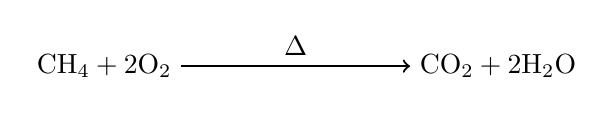
\begin{tikzpicture}
    \node (A) at (0,0) {\(\mathrm{CH_4 + 2O_2}\)};
    \node (B) at (5,0) {\(\mathrm{CO_2 + 2H_2O}\)};

    \draw[->, thick] (A) -- node[above] {\(\Delta\)} (B);
  \end{tikzpicture}
  \tagstructend
\end{center}
